\documentclass[10pt]{article}
\usepackage{icmlko}

\icmlmeta{IP 파운데이션 월드모델}{317}{풀링이 사는 것과 죽이는 것}{판 rho 중 얼마가 도메인 가로지르기에서 오나 --- 처음 쟀다. 두 얇은 도메인을 살리고 하나를 죽인다}

\begin{document}

\twocolumn[
\icmlheader

\begin{abstract}
노트 303$\sim$316이 열네 편에 걸쳐 ``빌림''을 쟀는데 \textbf{그 총량을 한
번도 안 쟀다.} 그 열네 편이 잰 것은 ``자기 라벨과 무관한 축을 끄면 얼마나
잃나''이고, 그건 빌림의 \emph{한 경로}이지 풀링 전체가 아니다. 직접 쟀다 ---
각 도메인을 \textbf{혼자} 적합하고(그 도메인의 학습 행만) 같은 유보로 채점해
지금 판과 견줬다. \textbf{답이 셈 방식에 따라 열세 배 벌어진다}: 같은 자
F6 이면 \textbf{$+$0.0040}, 최선 대 최선이면 $+$0.0120, 같은 자 F18 이면
\textbf{$+$0.0289}, 챔피언 대 혼자-F6 이면 $+$0.0519. \textbf{이 판 자신의
선택 규칙}(판 $\rho$ 로 정식화 하나를 고른다)을 양쪽에 그대로 적용하면
\textbf{$+$0.0289} 다. 그리고 그것이 어디서 오는지가 더 중요하다 ---
\textbf{도서 $+$0.2806}($t{=}{+}4.61$) · \textbf{시장팝업 $+$0.2493}
($t{=}{+}2.67$)이 전부고, 큰 도메인 다섯은 $-$0.013 $\sim$ $+$0.030 으로
아무것도 아니다. \textbf{그리고 아이돌은 $-$0.4964}($t{=}{-}2.01$) --- 혼자면
0.5977 인데 풀에 넣으면 0.1012 다. \textbf{풀링은 얇은 도메인을 살리는
장치이고, 같은 얇음이 희생자도 만든다.} 그리고 F6 에서는 \textbf{도서조차
혼자가 낫다}(0.3263 대 0.3108) --- F18 의 큰 이득은 \textbf{나무가 80행으로
못 적합하는 것}에서 온다.
\end{abstract}
]

\section{총량을 안 쟀다}

노트 303이 ``빌림''을 정의한 뒤 열네 편이 그것을 갈랐다 --- 도메인별(303 ·
312) · 정식화별(311) · 축별(313) · 채권자별(310 · 314). \textbf{그런데 그
모두가 같은 검사였다}: 자기 라벨과 무관한 축(``안 오른다'')을 끄면 얼마나
잃나. 축이 제 도메인에서도 유익하면 그 검사에 안 잡힌다.

\paragraph{직접 재는 법} 각 도메인을 \textbf{혼자} 적합한다 --- 그 도메인의
학습 행만 남기고 나머지 도메인의 학습 라벨을 지운다. 축은 그대로 둔다(축을
빼면 다른 실험이 된다). 같은 유보 행으로 채점한다.

\section{답이 넷이다}

\begin{figure*}[t]
\centering
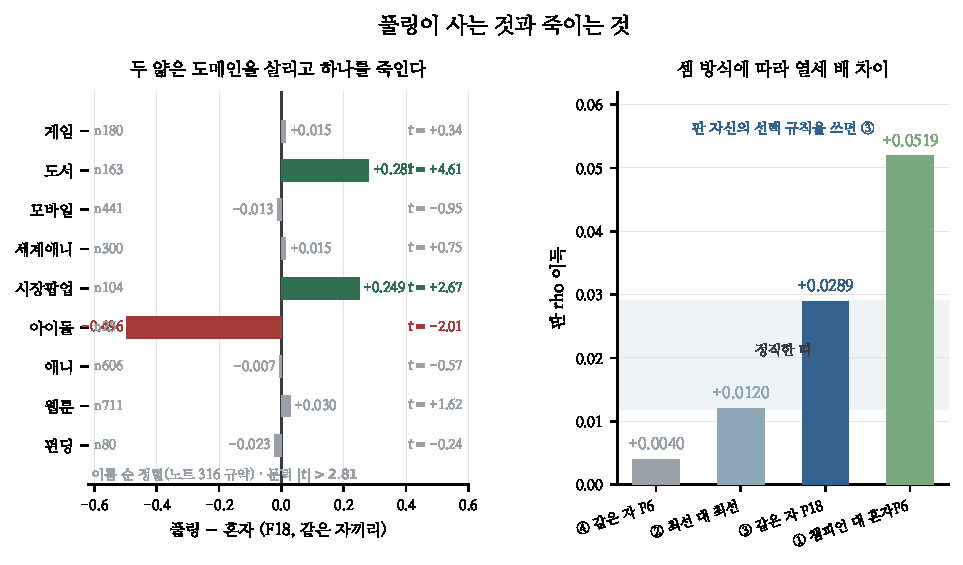
\includegraphics[width=\textwidth]{figs/pool.pdf}
\caption{왼쪽 --- 도메인별 풀링 이득(F18, 같은 자끼리, 이름 순).
오른쪽 --- 셈 방식 넷.}
\end{figure*}

\begin{center}\small
\begin{tabular}{lr}
\hline
셈 & 판 이득 \\
\hline
④ 같은 자 F6 & \textbf{$+$0.0040} \\
② 풀링 최선 대 혼자 최선 & $+$0.0120 \\
\textbf{③ 같은 자 F18} & \textbf{$+$0.0289} \\
① 챔피언 대 혼자-F6 & $+$0.0519 \\
\hline
\end{tabular}
\end{center}

\paragraph{어느 것이 맞나} \textbf{③ 이다.} 이 판은 판 $\rho$ 로 정식화
하나를 골라 전 도메인에 쓴다. 그 규칙을 \emph{양쪽에} 적용하면 --- 풀링
쪽도 혼자 쪽도 F18 을 고른다(혼자 판 F18 0.4527 $>$ F6 0.4297) --- 차가
$+$0.0289 다.

② 는 도메인마다 정식화를 유보로 골라 준 것이라 \textbf{혼자 쪽에 유리한
반칙}이다(유보로 고르면 안 된다, 노트 126). ① 은 챔피언 F18 이 이미 판
$\rho$ 로 뽑힌 것이라 \textbf{풀링 쪽에 유리}하다. \textbf{정직한 띠는
$+$0.012 $\sim$ $+$0.029} 이고 규칙을 지키면 $+$0.0289 다.

\section{어디서 오나 --- 그리고 어디서 잃나}

\begin{center}\footnotesize
\begin{tabular}{lrrrr}
\hline
도메인 & 유보 & 풀링 & 혼자 & $t$ \\
\hline
게임 & 180 & 0.5893 & 0.5748 & $+$0.34 \\
\textbf{도서} & 163 & \textbf{0.3895} & 0.1089 & \textbf{$+$4.61} \\
모바일 & 441 & 0.5464 & 0.5594 & $-$0.95 \\
세계애니 & 300 & 0.5475 & 0.5329 & $+$0.75 \\
\textbf{시장팝업} & 104 & \textbf{0.4098} & 0.1605 & \textbf{$+$2.67} \\
\textbf{아이돌} & 25 & \textbf{0.1012} & 0.5977 & \textbf{$-$2.01} \\
애니 & 606 & 0.4764 & 0.4837 & $-$0.57 \\
웹툰 & 711 & 0.4614 & 0.4317 & $+$1.62 \\
펀딩 & 80 & 0.2536 & 0.2766 & $-$0.24 \\
\hline
\end{tabular}
\end{center}

(팝업은 학습 16행이라 \textbf{혼자서는 점수가 없다} --- 0 으로 세지 않고
표에서 뺐다. 사전 등록의 미리 적는 실패 그대로다.)

\paragraph{살리는 둘} 도서 $+$0.2806($t{=}4.61$)과 시장팝업 $+$0.2493
($t{=}2.67$). \textbf{둘 다 학습 80 · 101행이다.} 문턱($|t|{>}2.81$)을 넘는
것은 도서 하나이고 시장팝업은 그 언저리다.

\paragraph{큰 다섯은 아무것도 아니다} 웹툰 $+$0.030 · 세계애니 $+$0.015 ·
게임 $+$0.015 · 애니 $-$0.007 · 모바일 $-$0.013. \textbf{절반이 음수다.}
판 무게의 78\%를 지는 도메인들이 풀링에서 아무것도 못 얻는다.

\paragraph{그리고 죽이는 하나} \textbf{아이돌 $-$0.4964}($t{=}{-}2.01$).
혼자 적합하면 0.5977 인데 풀에 넣으면 0.1012 --- 판에서 제일 낮은 도메인
점수가 \textbf{풀링 때문}이다. 유보 25행이라 문턱은 못 넘지만 크기가
이 표에서 제일 크다. \textbf{얇아서 살고 얇아서 죽는다.}

\section{그런데 F6 에서는 도서조차 혼자가 낫다}

\begin{center}\small
\begin{tabular}{lrr}
\hline
도서 & 풀링 & 혼자 \\
\hline
F18 (나무) & \textbf{0.3895} & 0.1089 \\
F6 (선형) & 0.3108 & \textbf{0.3263} \\
\hline
\end{tabular}
\end{center}

\textbf{F18 의 $+$0.28 이 통째로 나무의 표본 굶주림이다.} 나무는 80행으로
못 적합한다(\texttt{min\_samples\_leaf} 20 이면 잎이 넷)--- 그래서 0.1089 다.
선형은 80행으로 0.3263 을 낸다. \textbf{``혼자서는 못 한다''가 아니라
``나무로는 혼자서 못 한다''였다.}

그래도 \textbf{풀링-F18 0.3895 가 혼자-F6 0.3263 보다 높다} --- 순 이득
$+$0.063 은 남는다. 다만 \textbf{$+$0.28 이 아니라 $+$0.06} 이다.

\paragraph{그래서 판 이득의 정직한 읽기} F6 에서 판 이득이 $+$0.0040 인 것이
그 뜻이다 --- \textbf{선형에서는 풀링이 거의 아무것도 안 한다.} F18 의
$+$0.0289 중 상당 부분이 ``나무가 작은 도메인을 혼자 못 다룬다''이지
``도메인끼리 배울 것이 있다''가 아니다.

\section{그러면 이 판은 파운데이션인가}

\begin{center}\footnotesize
\begin{tabular}{ll}
\hline
말할 수 있는 것 & \\
\hline
풀링이 판을 올린다 & $+$0.012 $\sim$ $+$0.029 \\
이득은 얇은 둘에서 & 도서 · 시장팝업 (유보 267행, 10\%) \\
큰 다섯은 못 얻는다 & 절반이 음수 \\
얇은 하나는 크게 잃는다 & 아이돌 $-$0.50 \\
선형에서는 거의 0 & $+$0.0040 \\
\hline
\end{tabular}
\end{center}

\textbf{``여럿에서 배워 하나에 쓴다''는 일어난다} --- 도서와 시장팝업에서.
\textbf{그런데 그것이 판을 크게 올리지는 않고}(판의 90\%는 아무것도 안
얻는다) \textbf{선형에서는 사라진다.} 이 판의 파운데이션성은
\textbf{작고 · 얇은 도메인에 국한되고 · 정식화에 달렸다.}

\paragraph{남은 것}
\begin{center}\small
\begin{tabular}{ll}
\hline
갈래 & 왜 \\
\hline
아이돌은 왜 죽나 & 이 표에서 제일 큰 값이다 \\
얇은 도메인을 더 & 이득이 나는 유일한 자리 \\
정식화별 풀링 이득 & F6 0.004 대 F18 0.029 를 갈라 \\
팝업(혼자 점수 없음) & 풀링 아니면 아예 못 잰다 \\
\hline
\end{tabular}
\end{center}

\paragraph{규약} \textbf{반사실을 고를 때 양쪽에 같은 규칙을 써라.} 이
한 물음에 답이 넷 나왔고 열세 배 벌어졌다 --- 차이는 전부 ``혼자 쪽에
어떤 정식화를 줄 것인가''였다. \textbf{판이 챔피언을 고르는 규칙을 혼자
쪽에도 그대로 주는 것}이 유일하게 편향 없는 셈이다. 그리고 \textbf{총량을
한 번은 재라} --- 열네 편이 ``빌림''을 갈랐는데 그 열넷이 전부 한 경로만
보고 있었고, 총량을 재니 \textbf{선형에서는 0} 이었다.

\end{document}
